\documentclass[10pt, reqno]{article}
\usepackage[utf8]{inputenc}
\usepackage[margin = 1cm, a6paper, landscape]{geometry}
\usepackage{amsmath, amsfonts, amssymb, amsthm, graphicx}
\usepackage[ruled]{algorithm2e}
\usepackage{caption}

\usepackage{hyperref}
\usepackage[dvipsnames]{xcolor}
\hypersetup{colorlinks, linkcolor={MidnightBlue}, citecolor={MidnightBlue}, urlcolor={MidnightBlue}}

\usepackage{tikz}

\setlength{\parindent}{0pt}
\newcommand{\forceindent}{\leavevmode{\parindent=1em\indent}}
\numberwithin{equation}{section}

\newtheorem*{theorem*}{Theorem}
\newtheorem*{cor*}{Corollary}

\newcommand{\norm}[1]{\left\lVert#1\right\rVert}
\newcommand{\e}{\epsilon}
\newcommand{\w}{\omega}
\newcommand{\R}{\mathbb{R}}
\newcommand{\N}{\mathbb{N}}
\newcommand{\Q}{\mathbb{Q}}
\newcommand{\Z}{\mathbb{Z}}
\renewcommand{\ae}[1]{\text{ \hspace{5pt} a.e. #1}}

\begin{document}
%\pagestyle{empty}
\setlength{\footskip}{-1cm}
 

\title{Combining $l^1$ Penalization with Higher Moment Stability Constraints in Regression Models}
\author{Austin David Brown}
\date{\today}

%%%
% Slide
%%%
\maketitle

%%%
% Slide
%%%
\newpage
\section*{Motivation}

\begin{itemize}
\item In statistics and probability theory it is common to impose moment assumptions on a random variable $X : \Omega \to \R^n$ such as $E(\norm{X}^k) < \infty$ for $k \in \R$.

\item These constraints correspond to the $L^p$ spaces which allow control over the width and the height of such random variables.
This can be interpreted as imposing "stability" on the random variable $X$.

\item If statisticians so freely impose such constraints then we should build a tool to allow scientists and researchers to impose such constraints on their real problems.

\item  In this project, we build a package implements this idea.
The goal is not to create the best predicting method, but instead build a tool that will allow researchers to explore stability and what a "stable" solution to their problem may look like.
\end{itemize}

%%%
% Slide
%%%
\newpage
\section*{Geometric Motivation}
Consider for example an Elasticnet \cite{elasticnet} penalty $Q(x) = \frac{1}{2} |x| + \frac{1}{2} |y| + \frac{1}{2} |x|^2 + \frac{1}{2} |y|^2 \le 1$
shown on the left and a new penalty $P(x) = \frac{1}{2} |x| + \frac{1}{2} |y| + \frac{1}{2} |x|^4 + \frac{1}{2} |y|^4 \le 1$ shown on the right.

\vspace{.5cm}
\begin{center}
\begin{minipage}{.5\textwidth}
  \centering
  \includegraphics[width=.9\linewidth]{elasticnet.png}
\end{minipage}%
\begin{minipage}{.5\textwidth}
  \centering
  \includegraphics[width=.9\linewidth]{new_penalty_4_moment.png}
\end{minipage}
\end{center}
\vspace{.5cm}

It seems reasonable that a scientist may want the option to "bow" out the feasible set even more.

%%%
% Slide
%%%
\newpage
\section*{Penalizations}

Define these penalizations to try to impose more "stability" for scientists and researchers (try to extend the Elasticnet idea)

\[
P(\lambda) = \lambda \alpha_0 \norm{\beta}_1 + \lambda \sum_{k = 1}^{5} \alpha_k \norm{\beta}_{2k}^{2k} 
\]

\[
P'(\lambda) = \lambda \alpha_1 \norm{\beta}_1 + \lambda \alpha_2 \norm{\beta}_\infty 
\]

\[
P''(\lambda) = \lambda \alpha_1 \norm{\beta}_1 + \lambda \sum_{k = 2}^{10} \alpha_k \norm{\beta}_{k}
\]

where $\lambda \in \R_{+}$ and $\alpha$'s are convex combinations or use separate tuning parameters instead.
These are convex and $P$ is strongly convex!

%%%
% Slide
%%%
\newpage
\section*{Objective}

Let
\[
L_{\lambda}(\beta) = \frac{1}{2} \norm{y - X \beta}_2^2 + \lambda P(\beta)
\]
be the objective with $y \in \R^n$ centered, $X \in M_{n \times p}(\R)$ centered, and $\beta \in \R^p$.

\vspace{1cm}

\begin{itemize}
\item I only had time to do Euclidean loss but this can be extended.

\item I only had time to implement the first penalization, so consider only the first one from here on out.

\item I now know how to do the others actually.
\end{itemize}

%%%
% Slide
%%%
\newpage
\section*{The Plan}

\begin{itemize}

\item \textbf{glmnet} \cite{glmnet} uses coordinate descent, but the implementation cannot be used and a new algorithm needs to be used.

\end{itemize}

%%%
% Slide
%%%
\newpage
\section*{Algorithm Implementation 1}

\vspace{.5cm}
\begin{algorithm}[H]
\caption{Subgradient Coordinate Method}
Choose $\beta^0 \in \R^p$ and tolerance $\delta > 0$;

Set $k \gets 0$

\Repeat{Until the loss difference $\Delta L$ is less than $\delta$}{ 

  Set the step size $h^k \gets \frac{R}{\sqrt{1 + k}}$ for some $R > 0$ or use a constant step size.

  Permute $I = \{1, \ldots, p\}$

  \For {$i \in I$}{

    $\beta^{k + 1}_i \gets \beta^{k}_i - h^i g^i$ where $g^i \in (\partial L)_i$

  }

  $k \gets k + 1$
}

\end{algorithm}
\vspace{.5cm}

%%%
% Slide
%%%
\newpage
\section*{Drawbacks}

\begin{itemize}
\item Not a descent method. 

\item No good stopping criterion.

\item The stopping criterion is also expensive at $O(n^2)$ flops.

\item Convergence theory is worse.

\item Rarely produces sparse solutions really small values instead.

\end{itemize}


%%%
% Slide
%%%
\newpage
\section*{A Much Better Algorithm}

\vspace{.5cm}
\begin{algorithm}[H]
\caption{Proximal Gradient Coordinate Descent}
Choose $\beta^0 \in \R^p$ and tolerance $\delta > 0$;

Set $k \gets 0$

\Repeat{Until the Moreau-Yoshida mapping $M_{h_k, f} < \delta$}{ 

  Set the step size $h^k > 0$ with diminishing or line search.

  Randomly permute $I = \{1, \ldots, p\}$

  \For {$i \in I$}{

    $\beta^{k + 1}_i \gets (\textbf{prox}_{h^k L})_i ( \beta^k_i - h^k \langle X_i, y - X \beta \rangle )$

  }

  $k \gets k + 1$
}
\end{algorithm}
\vspace{.5cm}

%%%
% Slide
%%%
\newpage
\section*{Benefits}

\begin{itemize}
\item A descent method, so can do line search.

\item Good stopping criterion at $O(p^2)$ flops.

\item Convergence theory is unchanged from differentiable functions.

\end{itemize}

%%%
% Slide
%%%
\newpage
\section*{Architecture}

Written entirely in C++ for speed using Eigen \cite{eigen} and can be interfaced to many other popular languages.

\vspace{.5cm}
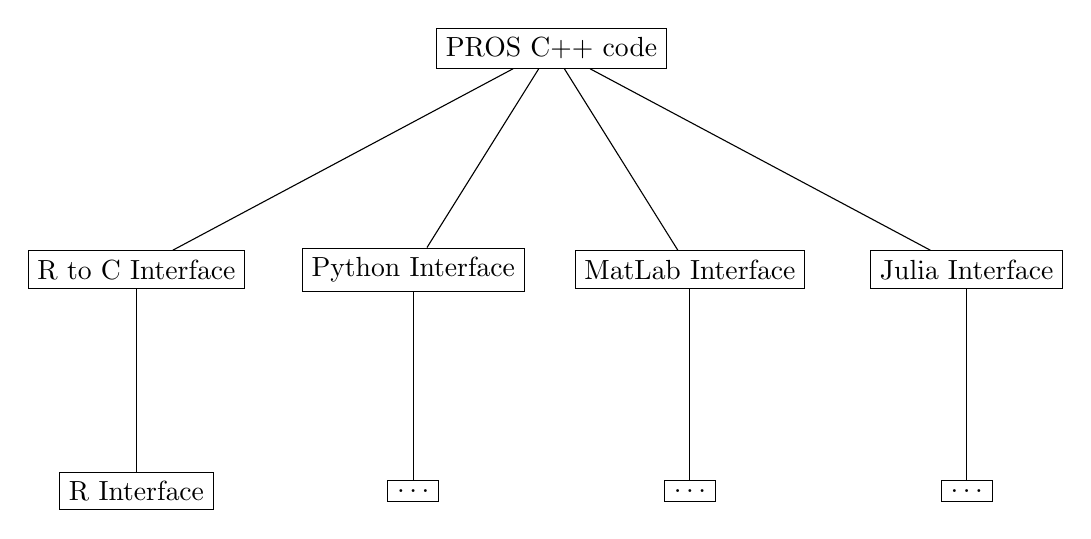
\begin{tikzpicture}[level distance=8em, sibling distance=10em,
  every node/.style = {shape=rectangle, draw, align=center}]]
  \node {PROS C++ code}
    child { node {R to C Interface} 
      child { node {R Interface} }
    }
    child { node {Python Interface} 
      child { node {$\ldots$} }
    }
    child { node {MatLab Interface} 
      child { node {$\ldots$} }
    }
    child { node {Julia Interface} 
      child { node {$\ldots$} }
    };
\end{tikzpicture}

%%%
% Slide 8
%%%
\newpage
\section*{Simple, Familiar Interface and No Dependencies}

A single fit function with prediction

\begin{verbatim}
> fit <- pros(X, y, alpha, lambda)
> predict(fit, new_X)
\end{verbatim}

A cross-validation fit function with prediction

\begin{verbatim}
> cv <- cv.pros(X, y, alpha)
> predict(cv, new_X)
\end{verbatim}

Ran out of time for plotting, but this would be cool.

No dependencies! I did not use RCPP.

%%%
% Slide
%%%
\newpage
\section*{Cross-Validation Implementation}

\vspace{.5cm}
\begin{algorithm}[H]
\caption{Warm Start Cross-Validation}
Choose a sequence of Langrangian dual variables $\lambda_1, \ldots, \lambda_N$, and initial value $\beta^0$.

Order $\lambda_{(1)}, \ldots, \lambda_{(N)}$ descending.

$\beta^{Warm} \gets \beta^0$ 

\For{$k \in 1, \ldots, N$}{

  $\beta^k \gets$ by Cross-Validation with $\lambda_{(k)}$ warm started with $\beta^{Warm}$.

  $\beta^{Warm} \gets \beta^k$
}

\end{algorithm}
\vspace{.5cm}

%%%
% Slide
%%%
\newpage
\section*{Penalized Regression on Steroids}


\begin{Large}
\href{https://github.com/austindavidbrown/pros}{Penalized Regression on Steroids on Github}
\end{Large}

\begin{itemize}
\item The name doesn't fit really since I only implemented 1 penalization

\item Talk about python prototype

\item Show how to download

\item Show the reference manual
\end{itemize}

%%%
% Slide
%%%
\newpage
\section*{Open Questions}

How to handle users and step sizes since we want to make it easy for users to use.

Backtracking line search?

%
% Bib
%
\newpage
\small
\begin{thebibliography}{1}

\bibitem{pros}
PROS. \href{https://github.com/austindavidbrown/pros}{github.com/austindavidbrown/pros}

\bibitem{boyd_proximalalgs}
Neal Parikh and Stephen Boyd. 2014. Proximal Algorithms. Found. Trends Optim. 1, 3 (January 2014), 127-239. DOI=10.1561/2400000003 http://dx.doi.org/10.1561/2400000003

\bibitem{wright_cd_algs}
Stephen J. Wright. 2015. Coordinate descent algorithms. Math. Program. 151, 1 (June 2015), 3-34. DOI=10.1007/s10107-015-0892-3 http://dx.doi.org/10.1007/s10107-015-0892-3

\bibitem{eigen}
Guennebaud, Gaël (2013). Eigen: A C++ linear algebra library (PDF). Eurographics/CGLibs.

\bibitem{glmnet}
Jerome Friedman, Trevor Hastie, Robert Tibshirani (2010). Regularization Paths for Generalized Linear Models via Coordinate Descent. Journal of Statistical Software, 33(1), 1-22. URL http://www.jstatsoft.org/v33/i01/.

\bibitem{elasticnet}
Zou, H. and Hastie, T. (2005). Regularization and variable selection via the elastic net. Journal of the Royal Statistical Society: Series B, 67, 301–320.

\bibitem{nesterov}
Yurii Nesterov. 2014. Introductory Lectures on Convex Optimization: A Basic Course (1 ed.). Springer Publishing Company, Incorporated.

\end{thebibliography}

\end{document}

